\section*{Marco Teórico}

\subsection*{Relación de Transformación}

En un autotransformador, parte de la energía se transfiere a través de un devanado común entre la bobina primaria y secundaria. La relación de voltajes entre el primario y el secundario de un autotransformador se determina como:

\begin{equation}
\frac{V_s}{V_p} = \frac{N_s}{N_p}
\end{equation}

Donde:
\begin{itemize}
    \item $V_s$: Voltaje en el lado secundario del autotransformador.
    \item $V_p$: Voltaje en el lado primario del autotransformador.
    \item $N_s$: Número de vueltas en la parte secundaria del devanado común.
    \item $N_p$: Número de vueltas en la parte primaria del devanado común.
\end{itemize}

En un autotransformador, la relación de voltaje depende de cuántas vueltas del devanado están involucradas en el secundario, en comparación con el primario. Es decir, la relación de voltaje es directamente proporcional a la cantidad de vueltas en cada parte del devanado.

\subsection*{Prueba de Vacío}

La prueba de vacío es un procedimiento utilizado para evaluar las pérdidas de núcleo o pérdidas de hierro del autotransformador. En esta prueba, el transformador se conecta al suministro eléctrico en su lado primario, aplicando el voltaje nominal, pero sin carga conectada al lado secundario. Al no haber carga, la corriente medida es pequeña y está compuesta principalmente por la corriente de magnetización, necesaria para excitar el núcleo del transformador.

Las pérdidas en este caso se deben principalmente a los efectos magnéticos en el núcleo, como las pérdidas por histéresis y las pérdidas por corrientes de Foucault, además de las pérdidas resistivas de los devanados. El objetivo principal de la prueba de vacío es medir la potencia de vacío, que es la potencia consumida por el transformador debido a las pérdidas de hierro, las cuales son constantes y no dependen de la carga. Estas pérdidas son importantes porque afectan la eficiencia global del transformador, ya que siempre están presentes, incluso cuando el transformador no está alimentando ninguna carga.


    \begin{figure}[ht!]
        \centering
        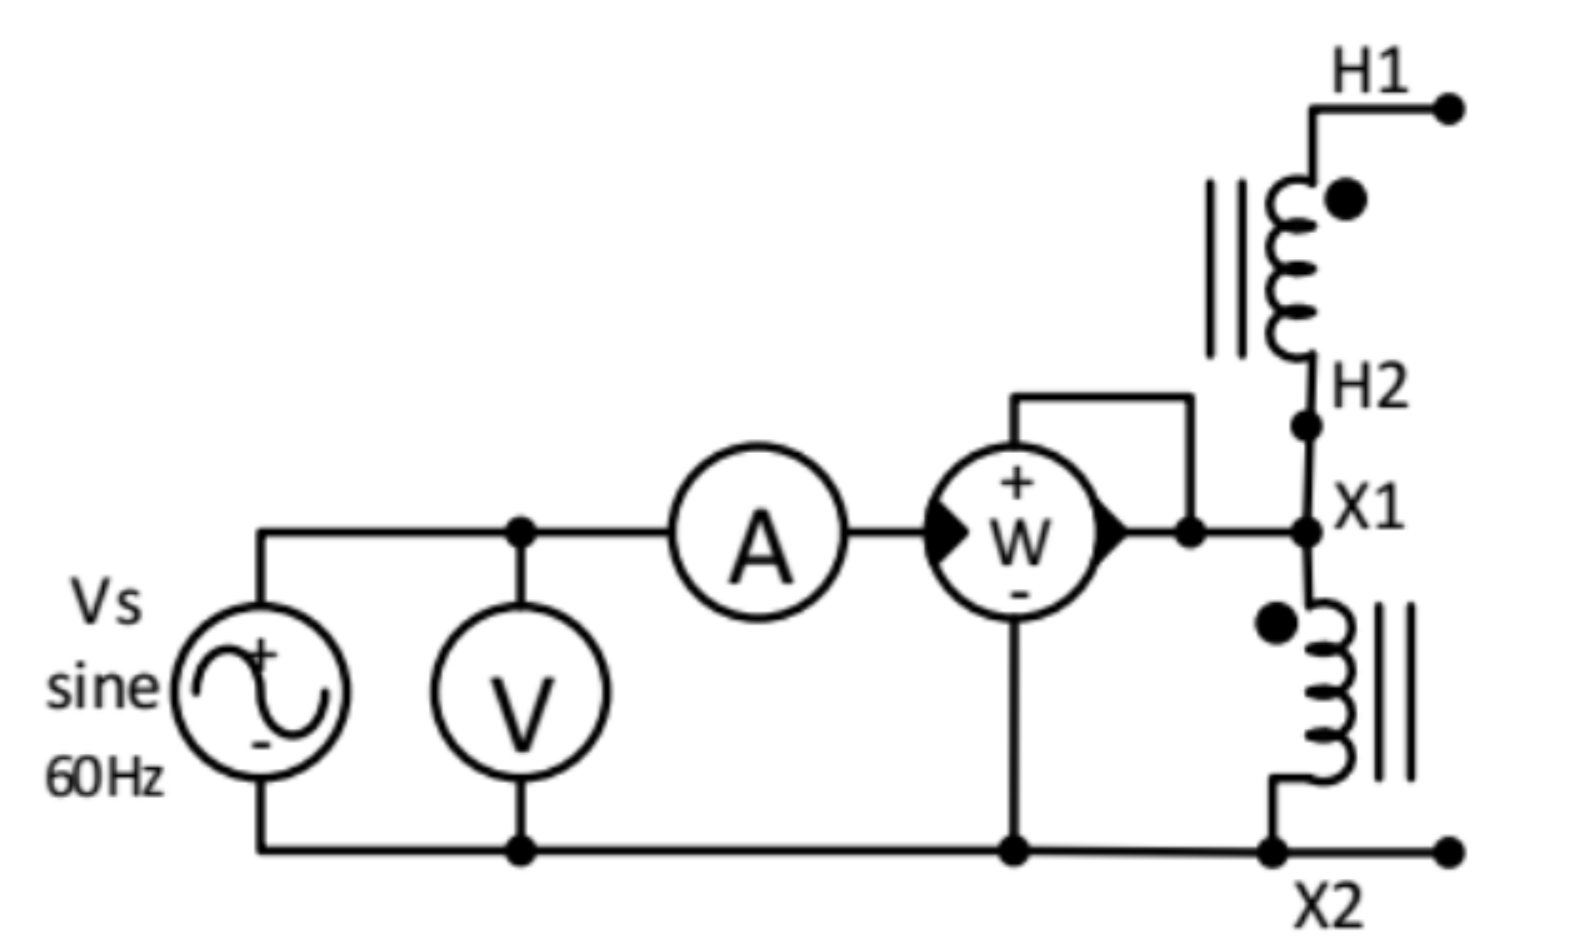
\includegraphics[width=0.48\textwidth]{fot/Prac4_vacio.png}
        \caption{Esquema de conexión del autotransformador a partir del transformador prueba de vacío. Fuente: PDF Práctica No. 4. Transformadores Monofásicos: Autotransformador.}
        \label{fig:EsquemaAutotransformadorvac}
    \end{figure}




\subsection*{Prueba de Corto Circuito}

La prueba de corto circuito se realiza para determinar las pérdidas de cobre y la impedancia de los devanados del autotransformador cuando este está bajo condiciones de carga. En esta prueba, el lado secundario del transformador se conecta a un cortocircuito, lo que provoca que la corriente de corto circuito fluya por los devanados secundarios. Al mismo tiempo, se aplica un voltaje reducido en el lado primario del transformador. Este voltaje es suficiente para generar la corriente de corto circuito requerida en el lado secundario, pero no es tan alto como para causar daños en el transformador.
\\
La corriente medida en esta prueba es proporcional a las pérdidas de cobre, que son pérdidas resistivas causadas por la resistencia de los devanados. Estas pérdidas dependen directamente de la corriente que circula por los devanados y son más altas cuando el transformador está bajo carga. A partir de esta prueba, se puede calcular la impedancia total del transformador, que incluye tanto la resistencia como la reactancia de los devanados. Esta impedancia es crucial para determinar el comportamiento del transformador bajo carga y para dimensionar adecuadamente el dispositivo según las necesidades de la red.
    \begin{figure}[ht!]
        \centering
        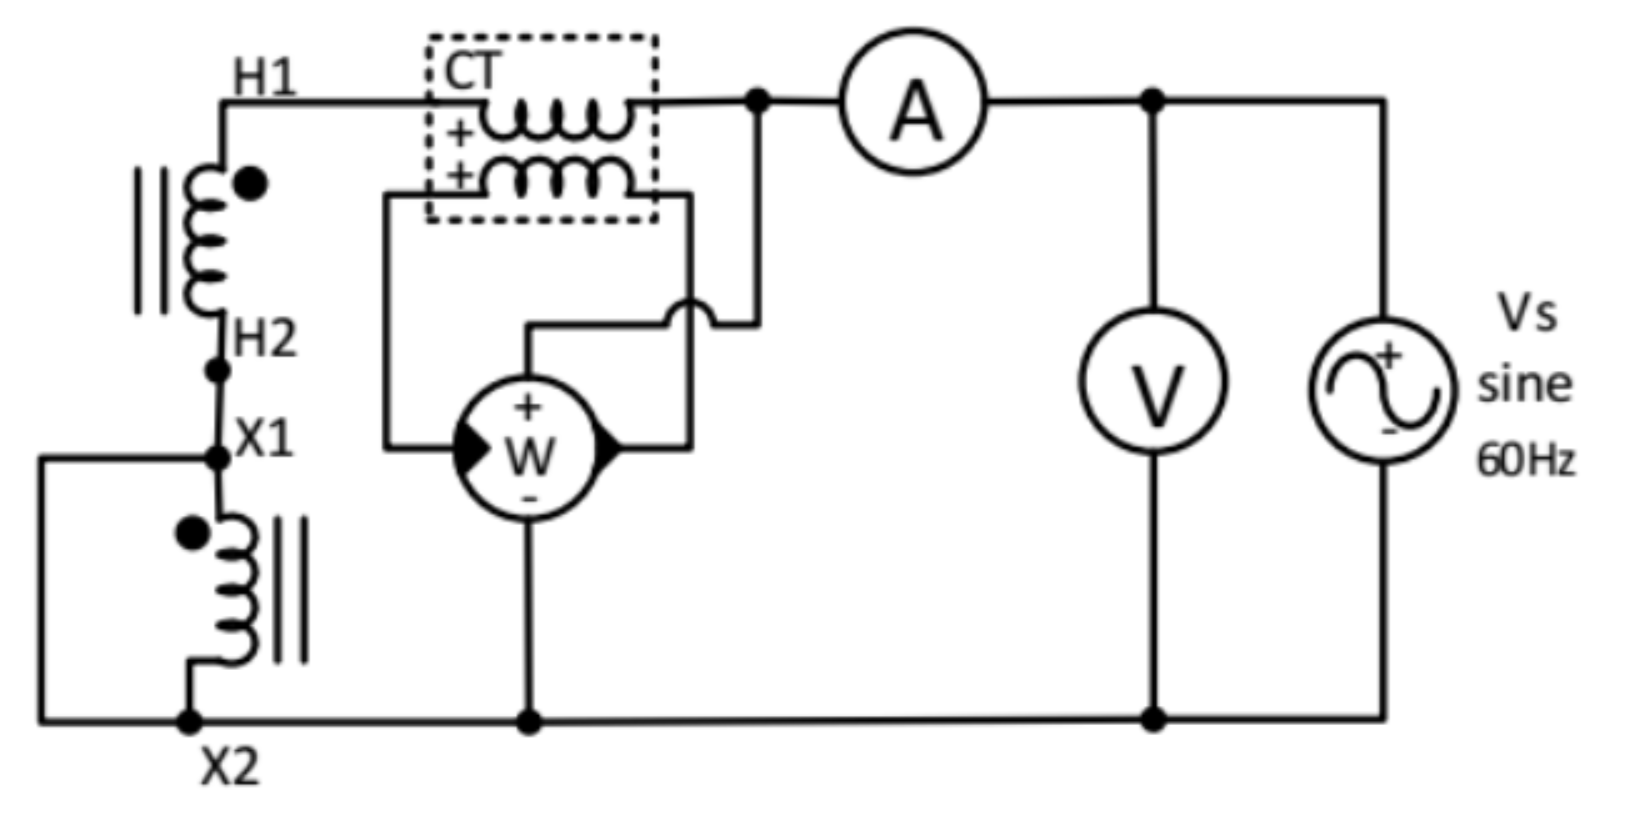
\includegraphics[width=0.48\textwidth]{fot/Prac4_corto.png}
        \caption{Esquema de conexión del autotransformador a partir del transformador prueba de cortocircuito. Fuente: PDF Práctica No. 4. Transformadores Monofásicos: Autotransformador.}
        \label{fig:EsquemaAutotransformadorcorto}
    \end{figure}


\subsection*{Prueba de Rendimiento}
La prueba de rendimiento se lleva a cabo para evaluar el comportamiento general del autotransformador cuando está operando con una carga conectada. El propósito de esta prueba es medir la eficiencia del transformador bajo condiciones de operación reales, es decir, cuando se le aplica una carga en su salida. Durante esta prueba, se mide tanto la potencia de entrada como la potencia de salida del transformador, así como las pérdidas totales que ocurren durante el proceso de transformación.
\\
Para realizar la prueba de rendimiento, se conecta el autotransformador a una carga conocida y se aplica el voltaje nominal en el lado primario. Se mide la potencia activa y reactiva tanto en el lado primario como en el secundario. Las pérdidas totales incluyen las pérdidas de hierro (que ya se determinaron en la prueba de vacío) y las pérdidas de cobre (que fueron determinadas en la prueba de corto circuito). La eficiencia del autotransformador se calcula como:


\begin{equation}
\eta [\%] = \frac{P_{\text{salida}}}{P_{\text{entrada}}} \times 100
\end{equation}

Este valor es fundamental para evaluar la efectividad del transformador al convertir la energía eléctrica de entrada en energía útil para la carga.

\subsection*{Regulación}

La regulación es un parámetro crítico en los transformadores, especialmente en los autotransformadores, y describe la capacidad del transformador para mantener un voltaje constante en su salida frente a las variaciones de carga. En términos simples, la regulación se refiere al cambio en el voltaje secundario cuando el transformador pasa de carga total a vacío.

La regulación de un transformador está estrechamente relacionada con las pérdidas de cobre y la impedancia de los devanados, ya que las variaciones de carga afectan la caída de tensión en los devanados. Cuando el autotransformador se carga, la corriente que fluye a través de los devanados genera una caída de tensión proporcional a la impedancia total del transformador, lo que reduce el voltaje de salida. La fórmula general para calcular la regulación de un transformador es:

\begin{equation}
\text{Regulación} = \frac{V_{\text{vacío}} - V_{\text{carga}}}{V_{\text{carga}}} \times 100
\end{equation}
